\documentclass[reqno]{amsart}
\usepackage{lipsum}
\usepackage{amsfonts}
\usepackage{amsmath}
\usepackage{amssymb}
\usepackage{clrscode3e}
\usepackage{tabularx}
\usepackage{graphicx}
\usepackage{floatrow}
\usepackage{tabularx}

\newtheorem{theorem}{Theorem}
\newtheorem{lemma}{Lemma}
\newtheorem{definition}{Definition}
\newtheorem{notation}{Notation}
\newtheorem{problem}{Problem}
\newtheorem{remark}{Remark}{\normalfont}
\newtheorem{proposition}{Proposition}
\newtheorem{corollary}{Corollary}
\newtheorem{example}{Example}
\theoremstyle{definition}
\newtheorem*{summary}{Summary}
\newtheorem*{solution}{Solution}
\newtheorem*{exercise}{Exercise}

\begin{document}
\author{Alvin Wang / Dayou Li / Tianjian Che / Xiaoyang Chi}
\title{Inflation Forecasting With Commodities}
\maketitle
\begin{abstract}
Inflation has not been a serious and persistent economic problem in developed country for decades. However, in the wake of the Covid-19 pandemic, fears of inflation have returned. Where is inflation headed, and how can we use what we know to predict where it will go in real time? The causes and effects the variations of inflation are raising peoples' concern. Today we try to use machine learning models in order to find a more accurate measurement method of nowcasting the inflation rates with pricing of commodities.
\end{abstract}
\section{Data collection and processing}
The raw historical data that used to feed our machine learning model can be sourced from Kaggle, which includes the daily prices of comodity (Gold, Palladium, Nickel, Brent Oil, Natural Gas and Wheat) from 2000 to March, 2022 and the CPI data of United States.\\
~\\

We focused on data cleaning as part of feature engineering. The removal of missing values (NaNs) might cause the decreasing of model interpretability and reliablity, so we filt each missing value with its next valid value. Besides, for the mixed frequency dataframe, we interpreted $X$ in days, and $Y$ in months, and then took monthly averages on $X$.\\
~\\

The following formula would be used to calculate year-to-year growth rate:
\begin{align*}
\mbox{Growth} = \frac{(\mbox{this year CPI}-\mbox{last year CPI})}{\mbox{last year CPI}}
\end{align*}

\begin{figure}[t]
\centering
\caption{Inflation}
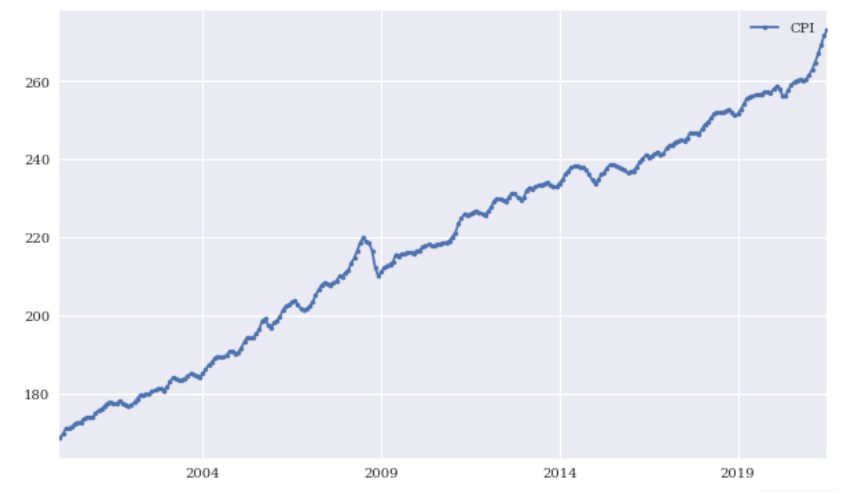
\includegraphics[scale=0.7]{inflation.png}
\end{figure}

\begin{figure}[t]
\centering
\caption{Year-to-Year Growth Rate of CPI}
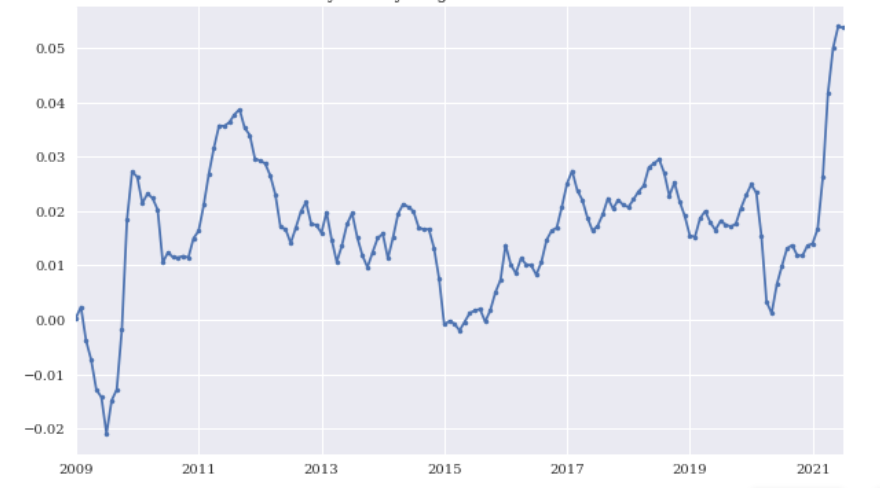
\includegraphics[scale=0.7]{growth.png}
\end{figure}


\newpage
\section{First attempt: Ordinary Linear Regression}
As the naivest and most intuitive method, we firstly applied OLS (ordinary least squares). The establishment of the model was relatively simple: firstly, we split the data set into training data set (before 2017) and testing data set (after 2017), and then ran the LinearRegression model from the sklearn library, which returned the following outcome.
\begin{figure}[h]
\centering
\caption{Linear Regression}
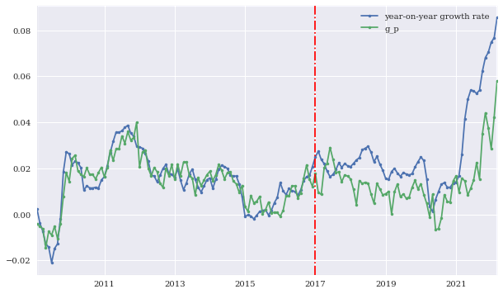
\includegraphics{LinearRegression.png}
\end{figure}
\newpage
\section{Linear regression with regularizations}
Adding LASSO or Ridge regularizations could be an effective way to reduce probability of overfitting, the following graphs shows the performanaces of adding LASSO regularization and Ridge regularization respectively.\\
~\\

\begin{figure}[h]
\centering
\caption{With Lasso Regularizations}
\includegraphics[scale=0.8]{LASSO.png}
\end{figure}

\begin{figure}[h]
\centering
\caption{With Ridge Regularizations}
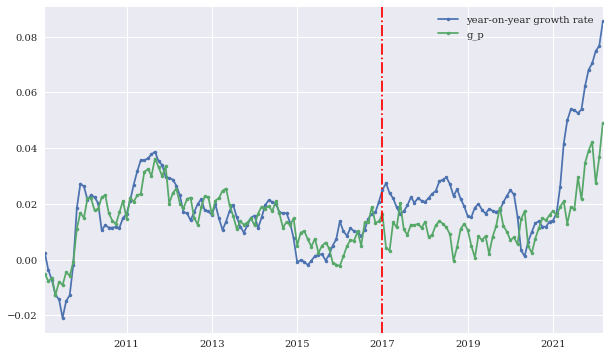
\includegraphics[scale=0.8]{Ridge.png}
\end{figure}
\newpage

\newpage
\section{Applying other machine learning models}
In this section, we tried to apply different machine learning models or parameter modifications as introduced in lectures, including LSTM, Multilayer Perceptron, Random Forest, Decision Tree and XGBoost.

\begin{figure}[h]
\centering
\caption{LSTM}
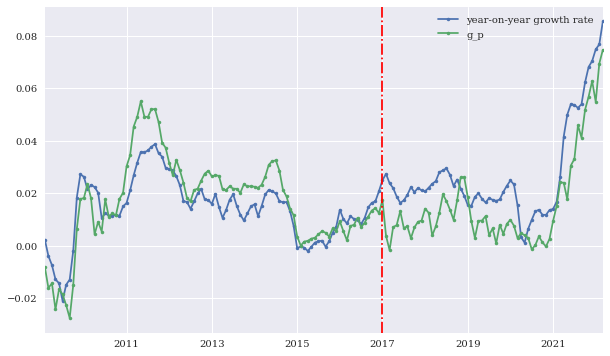
\includegraphics[scale=0.8]{LSTM.png}
\end{figure}

\begin{figure}[h]
\centering
\caption{Multilayer Perceptron with 10 layers}
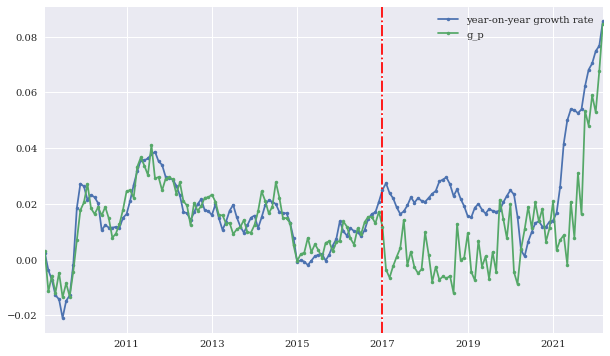
\includegraphics[scale=0.8]{Multilayer Perceptron.png}
\end{figure}

\begin{figure}[h]
\centering
\caption{Random Forest}
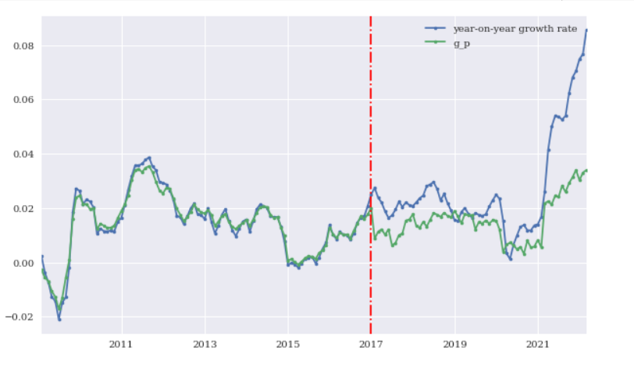
\includegraphics[scale=0.8]{Random Forest.png}
\end{figure}

\begin{figure}[h]
\centering
\caption{Decision Tree}
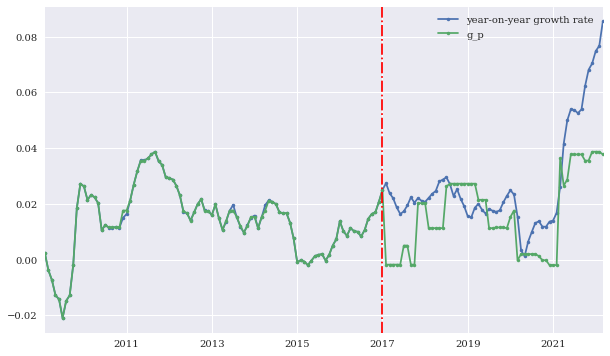
\includegraphics[scale=0.78]{Decision Tree.png}
\end{figure}

\begin{figure}[t]
\centering
\caption{XGBoost}
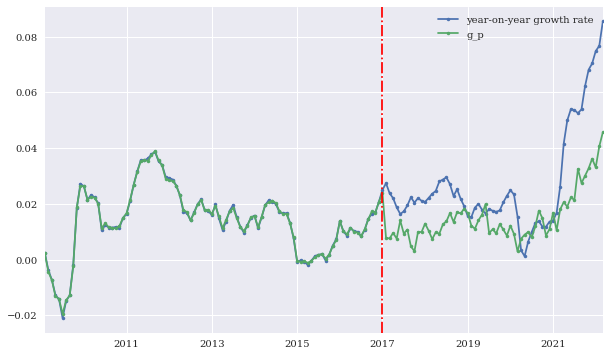
\includegraphics[scale=0.8]{XGBoost.png}
\end{figure}
~\\
~\\
~\\
~\\
~\\
~\\
~\\
~\\
~\\
~\\
~\\
~\\
~\\
~\\
~\\
~\\
~\\
~\\

\section{Forcasting Summary}
As our model summary, the following table generates MSEs for each machine
learning model we chose.
\begin{table}[h]
\begin{center}
\caption{Model Summary}
\begin{tabular}{|l|l|l|}
\hline
& Training MSE & Testing MSE\\
\hline
OLS & $2.9104948516751224 \times 10^{-5}$ & $0.0003298666400212202$ \\
\hline
LassoCV & $5.0932319589503475 \times 10^{-5}$ & $0.00035088866067721177$ \\
\hline
RidgeCV & $3.68902460248577\times10^{-5}$ & $0.00033034868436919413$\\
\hline
LSTM & $6.995119679684246\times 10^{-5}$ & $0.00017586422637605402$ \\
\hline
MLP & $2.383843843916805\times 10^{-5}$ & $0.0004979056514379927$ \\
\hline
Random Forest & $3.929795329486218\times 10^{-6}$ & $0.00029031614677209805$ \\
\hline
Decision Tree & $1.8067843114297657\times10^{-7}$ &  $0.00028472309805151636$\\
\hline
XGB & $2.0120924594331378\times 10^{-7}$ & $0.0002871991363157281$ \\
\hline
\end{tabular}
\end{center}
\end{table}

~\\
~\\
~\\

\section{Nowcasting summary}
The following graphs generate the nowcasting outcomes and LSTM result.

\begin{figure}[t]
\centering
\caption{SMA outcome}
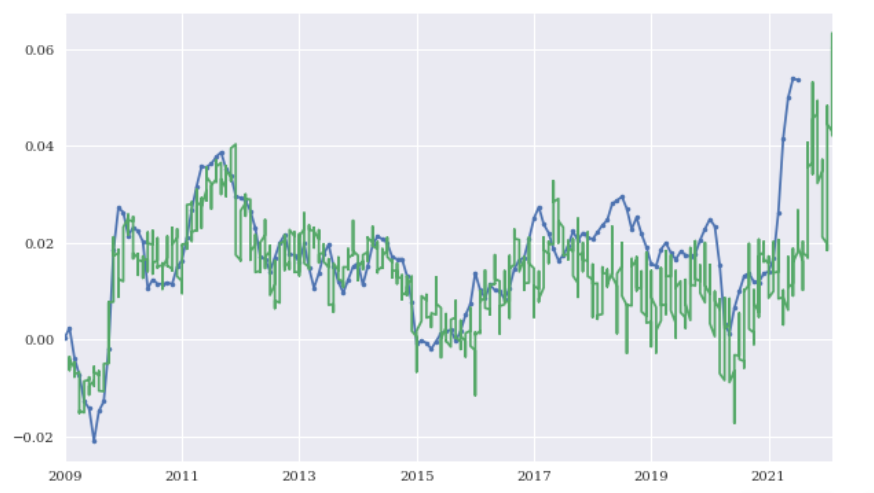
\includegraphics[scale=0.8]{SMA.png}
\end{figure}

\begin{figure}[t]
\centering
\caption{EMA outcome}
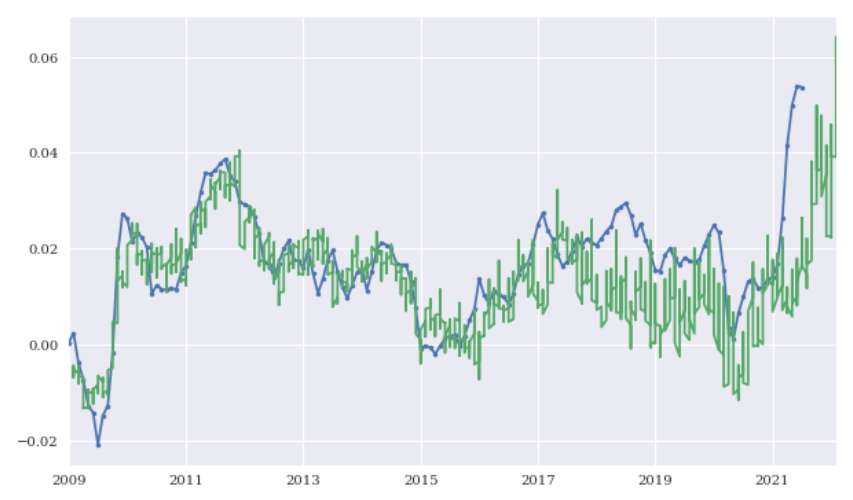
\includegraphics[scale=0.8]{EMA.png}
\end{figure}

\begin{figure}[t]
\centering
\caption{LSTM result}
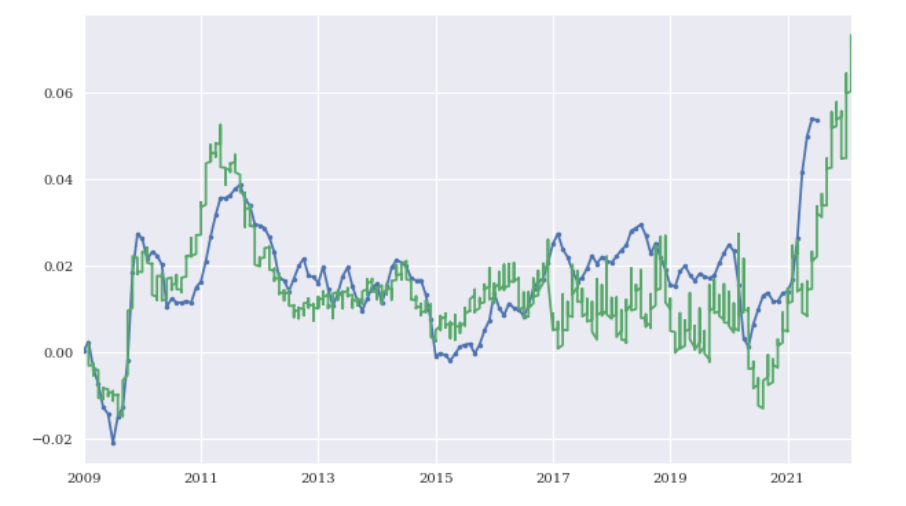
\includegraphics[scale=0.8]{LSTM2.png}
\end{figure}
\end{document} 